\chapter{Controleren van consistentie}\label{sec:consistentie}
In dit hoofdstuk treden we meer in detail over hoe we klassediagrammen voorstellen in FO($\cdot$). Daarvoor willen we een specifieke vorm van logische theorie automatisch laten genereren. In deze theorie\"en staan \textbf{objecten} centraal. Deze objecten zijn instanties van een klasse die voorkomt in het beschouwde diagram, hebben exact de attributen en operaties van die klasse en maken deel uit van exact die relaties die het diagram voorschrijft voor die klasse.

Het merendeel van het werk in dit hoofdstuk bestaat erin om de methode om klassediagrammen te vertalen naar eerste-orde-predicatenlogica ge\"introduceerd in \cite{BerardiDaniela2005RoUc} aan te passen om gebruik te maken van logische types zoals gedefinieerd in FO($\cdot$).

Aan de hand van volgend voorbeeld zullen we illustreren welke regels we gebruiken om een theorie op te bouwen:

\begin{figure}[H]
	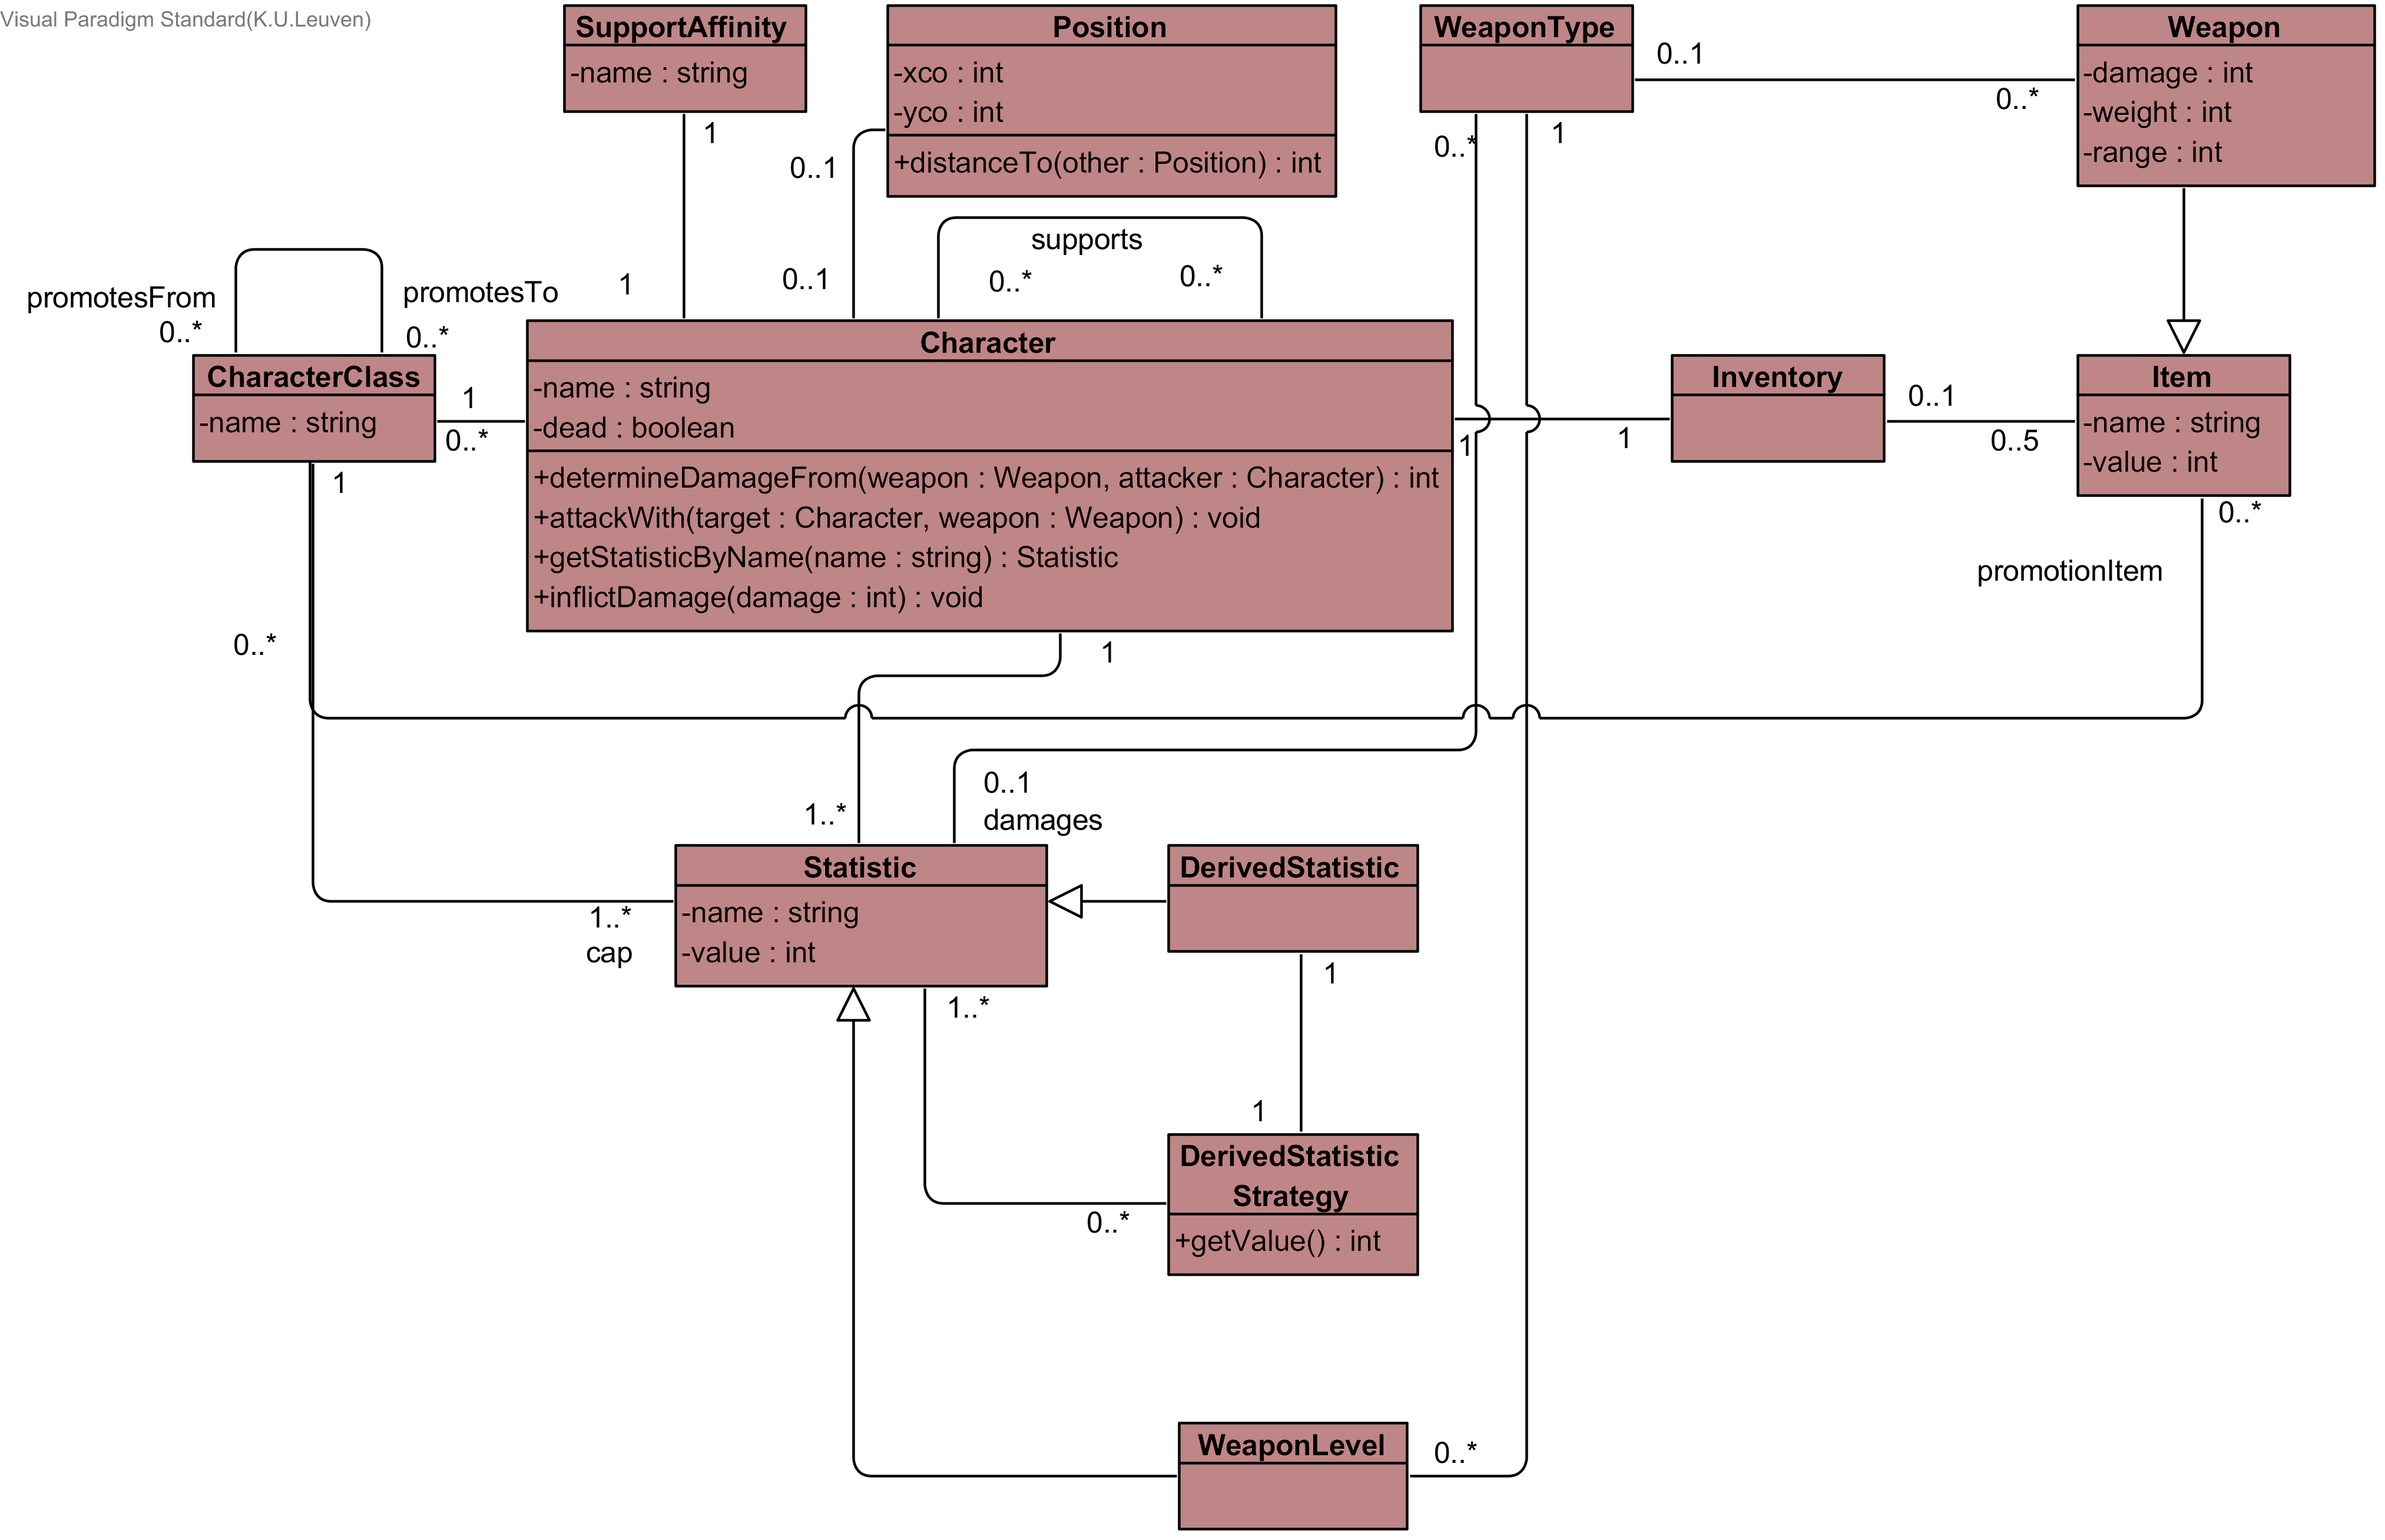
\includegraphics[width=0.95\textwidth]{chap-consistentie/diagram-voorbeeld.png}
	\caption{Leidend voorbeeld van een klassediagram}
	\label{fig:diagram-voorbeeld}
\end{figure}

Meer bepaald willen we uitdrukken welke \textbf{klasses} er bestaan in het diagram waarvan een object een instantie kan zijn, welke \textbf{attributen} en \textbf{operaties} elke klasse bevat, welke \textbf{associaties} er bestaan tussen de verscheidene klasses en welke \textbf{klassehi\"erarchie\"en} er bestaan.

\section{Logische types voor objecten}
We moeten een manier hebben om objecten te benoemen in een theorie en te specificeren tot welke klasse die objecten behoren. Voor beide van deze noden zijn logische types geschikt. We voegen voor elke klasse een logisch type toe aan het vocabularium. Er is een logisch type \textit{Character}, een logisch type \textit{Position}, etc.

\section{Voorstellen van attributen}
Voor elk attribuut voegen we een binair predicaat toe waarvan de naam beantwoordt aan het patroon: \textit{Klassenaamattribuutnaam}. Voor klasse \textit{Character} en attribuut \textit{name} resulteert dit dus in het predicaat \textit{Charactername/2}. Het eerste argument van dit predicaat is een \textit{Character}. Het type van het tweede argument hangt af van wat er in het diagram staat: Als het een primitief type is zoals \textit{string} of \textit{int}, zal dat ook het type zijn van het tweede predicaat; in het andere geval is het type van het tweede argument het overeenkomstig logisch type voor die klasse. Op deze manier wordt afgedwongen dat elk argument van het predicaat van het juiste type is.
De signatuur van \textit{Charactername/2} is daarom \textit{Charactername(Character, string)}.
Voor elk attribuut wordt ook een regel omtrent multipliciteit afgeleid. Zij \textit{lowerBound} de ondergrens en \textit{upperBound} de bovengrens. Dan is de meest algemene vorm van deze regel als volgt:
	
\begin{align*}
	\forall{o1}[KlasseType](lowerBound \geq \#\{o2 [AttribuutType] : \\ Klasseattribuutnaam(o1,o2)\} \geq upperBound).
\end{align*}
	
waarbij \textit{lowerBound} wordt weggelaten als deze $0$ is en \textit{upperBound} wordt weggelaten als deze $*$ is. Indien beide van deze voorwaarden gelden, wordt er geen regel afgeleid betreffende de multipliciteit van het attribuut. Als $lowerBound = upperBound$, wordt deze regel in de plaats:
	
\begin{align*}
	\forall{o1}[KlasseType] \exists_{=upperBound}{o2}[AttribuutType](Klassenaamattribuutnaam(o1,o2)).
\end{align*}
	
Voor \textit{Charactername/2} wordt daarom afgeleid:
	
\begin{align*}
	\forall{o1}[Character]\exists!{x}[string](Charactername(o,x)).
\end{align*}

\section{Voorstellen van operaties}
Voor elke operatie voegen we een predicaat toe dat beantwoordt aan volgend patroon: \textit{Klassenaamoperatienaam/(m+2)}, waarbij $m$ het aantal argumenten dat als invoer wordt meegegeven aan de operatie. De signatuur ziet eruit als \\ \textit{$Klasseoperatienaam(o,p_1,\ldots,p_m,r)$}, waarbij \textit{o} het object van het logisch type overeenkomstig de klasse waarvan de operatie deel is, \textit{$p_1$} \ldots \textit{$p_m$} de argumenten en \textit{r} het resultaat van de oproep van de operatie op het object \textit{o} met de gegeven argumenten. Indien er geen argumenten zijn, ziet de signatuur eruit als \textit{Klassenaamoperatienaam(o,r)}. Voor \textit{determineDamageWeaponFrom(Weapon)} van \textit{Character} wordt dit dus \textit{CharacterdetermineDamageFrom(Character,Weapon,int)}.

We moeten ervoor zorgen dat elke combinatie van object waarop de operatie wordt opgeroepen en mogelijke invoerparameters \'e\'en enkel resultaat is. Daarom leiden we regels af van de vorm:

\begin{align*}
	&\forall{o}[KlasseType]\forall{p_1}[ParameterType_1]\ldots\forall{p_m}[ParameterType_m]
	\\
	&\exists!{r}[ResultaatType](Klassenaamoperatienaam(o,p_1,\ldots,p_m,r)).
\end{align*}
	
De invulling voor \textit{CharacterdetermineDamageFrom(Character,Weapon,int)} wordt:
	
\begin{align*}
	&\forall{o}[Character\forall{p_1}[Weapon]\exists!{r}[int](CharacterdetermineDamageFrom(o,p1,r)).
\end{align*}

\section{Voorstellen van associaties}
Voor elke associatie voegen we een predicaat toe dat beantwoordt aan volgend patroon: \textit{$ClassOneand\ldots{}andClassM/m$}, waarbij \textit{m} de ariteit van de associatie. Voor de associatie tussen \textit{Inventory} en \textit{Item} wordt dit dus \textit{InventoryandItem(Inventory,Item)}.

De multipliciteit voor elke rol moet worden uitgedrukt. Voor alle $o_l$ waarvoor $1 \leq l \leq m$ wordt een regel toegevoegd van de volgende vorm:\\

Zij $lowerBound_l$ de ondergrens en $upperBound_l$ de bovengrens:
\begin{align*}
	&\forall{c_1}[Klasse_1]\ldots\forall{c_m}[Klasse_m](lowerBound_l \leq
	\\
	&\#\{o_l[Klasse_l] : ClassOneand\ldots{}ClassM(c_1,\ldots,o_l,\ldots,c_m)\} \leq upperBound_l).
\end{align*}
	
waarbij de \textit{c} met index \textit{l} overgeslagen wordt. Indien de ondergrens gelijk is aan $0$ of de bovengrens gelijk is aan $*$ worden dezen weggelaten. Als beide voorwaarden gelden, wordt voor deze \textit{l} geen regel afgeleid. Indien $lowerBound_l = upperBound_l$ wordt in de plaats afgeleid:
	
	\begin{align*}
	&\forall{c_1}[Klasse_1]\ldots\forall{c_m}[Klasse_m] \exists_{=upperbound_l}o_l[Klasse_l](ClassOneand\ldots{}andClassM\\&(c_1,\ldots,o_l,\ldots,c_m)).
	\end{align*}
	
	Voor \textit{InventoryandItem/2} worden de volgende regels afgeleid:
	
\begin{align*}
		\forall{o_2}[Item](\#{o_1[Inventory]: InventoryandItem(o_1,o_2)} \leq 1).
\end{align*} 
		
\begin{align*}
		\forall{o_1}[Inventory](\#{o_2[Item]: InventoryandItem(o_1,o_2)} \leq 5).
\end{align*}

\section{Voorstellen van klassehi\"erarchi\"een}\label{sec:hierarchies}
Aangezien FO($\cdot$) een getypeerde logica is, is het eenvoudig om klassehi\"erarchie\"een voor te stellen. Als volgens het diagram klasse \textit{X} een subklasse is van klasse \textit{Y}, dan is het voldoende om in het uitvoervocabularium te noteren dat logisch type \textit{Y} een supertype is van logisch type \textit{X}. Het is mogelijk om op die manier een keten van overervingsrelaties te modelleren en zo een hi\"erarchie te verkrijgen. In IDP in het bijzonder is het mogelijk dat een logisch type een subtype is van meer dan \'e\'en type, dus kan men ook meervoudige overerving modelleren.

Dit heeft echter een gevolg voor interpretaties van het logisch type overeenkomstig met een superklasse in een mogelijke structuur volgens het uitvoervocabularium. Indien klasse \textit{Z} een subklasse is van klasse \textit{X} uit de vorige paragraaf, dan moeten alle objecten die behoren tot klasse \textit{Z} ook behoren tot klasse \textit{X}, en zo ook moeten alle objecten die behoren tot klasses \textit{Z} en \textit{X} behoren tot klasse \textit{Y}.

Het is mogelijk om de eindgebruiker dit werk te besparen en automatisch de geschikte interpretaties te laten berekenen door af te stappen van een logisch type voor elke klasse en in de plaats twee nieuwe logische types te introduceren: Een algemeen logisch type voor objecten, \textit{Object}; en een \textit{constructed type}\cite{DeCatBroes2014PLaa} dat voor elke klasse in het diagram een overeenkomstig object heeft, \textit{ClassObject}.

Om lidmaatschap van een klasse uit te drukken, zijn er verder twee nieuwe predicaten nodig: \textit{RuntimeClass(ClassObject, Object)}, wat voor elk object uitdrukt tot welke klasse precies het behoort; en \textit{StaticClass(ClassObject, Object)}, wat uitdrukt tot welke klasses een object behoort als gevolg van de klassehi\"erarchie\"en in het diagram.

Er zijn ook twee predicaten nodig om overervingsrelaties tussen klasses te modelleren: \textit{IsDirectSupertypeOf(ClassObject, ClassObject)} om directe overervingsrelaties voor te stellen; en \textit{IsSupertypeOf(ClassObject, ClassObject)} dat de transitieve sluiting voor \textit{IsDirectSupertypeOf} voorstelt. Aangezien het in predicatenlogica onmogelijk is om een algemene voorstelling voor transitieve sluitingen uit te drukken, maken we gebruik van inductieve definities\cite{DeCatBroes2014PLaa}:

\begin{align}
\{
\nonumber &\forall{x}[ClassObject]\forall{y}[ClassObject](IsSupertypeOf(x,y) \leftarrow \\ &IsDirectSupertypeOf(x,y)).\label{def:tc1} \\
\nonumber &\forall{x}[ClassObject]\forall{y}[ClassObject](IsSupertypeOf(y,x) \leftarrow \\
&\exists{z}(IsSupertypeOf(y,z) \land IsSupertypeOf(z,x))).\label{def:tc2}
\}
\end{align}

Zin \ref{def:tc1} maakt gebruik van \textit{IsDirectSupertypeOf/2} om een basisgeval voor \textit{IsSupertypeOf/2} op te stellen. Zin \ref{def:tc2} bouwt dan verder de hi\"erarchie\"en op.

We maken in een tweede definitie gebruik van \textit{IsSupertypeOf/2} om \textit{StaticClass/2} in te vullen:

\begin{align*}
\{
&\forall{x}[ClassObject]\forall{o}[Object](StaticClass(x,o) \leftarrow RuntimeClass(x,o)). \\
&\forall{x}[ClassObject]\forall{y}[ClassObject]\forall{o}[Object](StaticClass(y,o) \leftarrow \\ &RuntimeClass(x,o) \land IsSupertypeOf(y,x)).
\}
\end{align*}

In een aparte definitie lijsten we de invulling voor \textit{IsDirectSupertype/2} gebaseerd op het diagram op. Voor het diagram in figuur \ref{fig:diagram-voorbeeld} wordt dit:

\begin{align*}
\{
IsDirectSupertypeOf(Statistic,Weaponlevel) \leftarrow .\\
IsDirectSupertypeOf(Statistic,DerivedStatistic) \leftarrow .\\
IsDirectSupertypeOf(Item,Weapon) \leftarrow .\\
\}
\end{align*}

We hebben echter niet voor deze aanpak gekozen voor twee redenen.
Attribuutpredicaten, operatiepredicaten en associatiepredicaten zouden logisch type \textit{Object} als argumenten moeten hebben. Dit betekent dat er nieuwe regels nodig zijn die afdwingen dat die objecten van het juiste type zijn. Grotere theorie\"en leiden tot een grotere rekentijd en geheugengebruik bij de uitvoering van redeneertaken.
De multipliciteitsregels zouden ook herschreven moeten worden om gebruik te maken van \textit{StaticClass}. Dit maakt zinnen over de hele lijn langer en zorgt ervoor dat ze moeilijker te begrijpen zijn.

\parbreak

In hoofdstuk \ref{sec:rol-idp} wordt de logische theorie die automatisch gegenereerd werd volgens de regels opgelijst in dit hoofdstuk weergegeven en wordt ook uitgelegd hoe die theorie wordt gebruikt om de consistentie van het diagram te controleren.